\begin{block}{Detecting 1D SPT Order}
\vskip1cm
If $U_g$ is a global symmetry and $\ket{\psi}$ is translationally invariant, then the MPS representation satisfies:

\begin{figure}[h]
    \centering
    \scalebox{1}{
    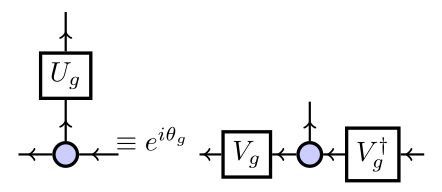
\includegraphics{diagrams/group_sym.png}
    }
\end{figure}

Boundary conditions on a MPS can be represented by a matrix $B$ which acts like: 

\begin{figure}[h]
    \centering
    \scalebox{1}{
    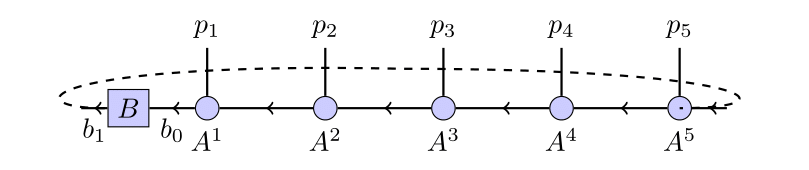
\includegraphics{diagrams/mpsbc.png}
    }
\end{figure}

With PBC ($B=I$) , the group action leaves the state invariant. 

With OBC ($B = \ket{i}\bra{i}$), the group action rotates between states that differ only near the boundary; these edge states transform as $V_g \otimes V_g^{\dagger}$. 

$V_g$ represents the group projectively. Equivalence classes of projective representations (enumerated by $H^2(G; U(1))$) classify 1D SPT phases.

\end{block}